\documentclass[11pt,a4paper]{article}

\usepackage[T1]{fontenc}
\usepackage[utf8]{inputenc}
\usepackage{lmodern}
\usepackage[a4paper,margin=2.4cm]{geometry}
\usepackage{amsmath,amssymb}
\usepackage{graphicx}
\usepackage{booktabs}
\usepackage{xcolor}
\usepackage{hyperref}

\definecolor{asd}{HTML}{DF756C}
\definecolor{td}{HTML}{3F8FC5}
\definecolor{ink}{HTML}{1B2433}
\hypersetup{colorlinks=true,linkcolor=ink,citecolor=ink,urlcolor=td}

\title{The Shape of Gaze:\\
Persistent Homology of ASD and Typically Developing\\
Fixation Patterns in Saliency4ASD}
\author{Shengkai Sun \and Xiaoye Ma}
\date{SF2956 Topological Data Analysis\\1 November 2026}

\newcommand{\ASD}{\textsc{asd}}
\newcommand{\TD}{\textsc{td}}
\newcommand{\R}{\mathbb{R}}

\begin{document}
\maketitle

\begin{abstract}
We investigate whether persistent homology captures systematic differences
between fixation locations of children with autism spectrum disorder (\ASD)
and typically developing controls (\TD) viewing the same static images.  The
public Saliency4ASD training release contains 300 stimuli and group-specific
scanpath files.  Because stable participant identifiers are unavailable, the
analysis unit is a matched stimulus--group point cloud rather than an
individual child.  For each eligible stimulus, 60 valid two-dimensional
fixation centres are sampled without replacement from each group, with 20
repetitions.  Coordinates are scaled by the image diagonal, and
Vietoris--Rips persistent homology is computed in dimensions 0 and 1.  The 20
repetitions are first averaged within stimulus; 287 matched stimuli are then
used for group comparison.  \ASD{} point clouds have higher spatial dispersion
and higher total $H_0$ persistence than \TD{} clouds.  The group-mean $H_0$
stable-rank curve is consequently higher and decays more slowly for \ASD.
$H_1$ summaries also differ, but their effects are smaller and more sensitive
to sampling.  The strong relation between $H_0$ total persistence and ordinary
spatial dispersion indicates that the primary topological result mainly
expresses a robust multiscale form of gaze dispersion.  The findings are
stimulus-level and exploratory; they do not constitute participant-level
diagnostic evidence.
\end{abstract}

\section{Introduction}

Eye-tracking data are often reduced to fixation counts, average coordinates,
or predefined areas of interest.  These summaries can miss how fixation
locations are arranged across several spatial scales.  Topological data
analysis (TDA) offers a complementary description: instead of selecting one
clustering radius, persistent homology follows connected components and holes
as the distance threshold changes.

This project asks:
\begin{quote}
Can persistent homology detect systematic differences between the spatial
distributions of \ASD{} and \TD{} group fixations when both groups view the
same static image?
\end{quote}
The primary outcome is finite $H_0$ persistence, which describes how spatial
components merge.  $H_1$ is retained as an exploratory description of holes
in the unordered point cloud.  The project analyses spatial coordinates only;
fixation duration and temporal order are deliberately excluded.

\section{Data and analysis unit}

The Saliency4ASD training data contain 300 natural-scene stimuli viewed by 14
children with ASD and 14 typically developing children aged 5--12
\cite{duan2019}.  Each stimulus has one \ASD{} and one \TD{} scanpath file.
The released files contain fixation index, position, and duration.  A reset of
the index marks a new anonymous scanpath segment, but there is no stable
participant identifier that can be linked reliably across all stimuli.

We therefore pool valid fixation centres within image and group.  For stimulus
$i$ and group $g\in\{\ASD,\TD\}$, the point cloud is
\[
X_{i,g}=\{(x_1,y_1),\ldots,(x_n,y_n)\}\subset\R^2.
\]
Each image supplies a matched \ASD--\TD{} comparison.  Individual fixations
are observations used to construct a point cloud, not independent subjects.
Likewise, the 20 random subsamples described below are Monte Carlo
repetitions, not additional experimental units.

\section{Methods}

\subsection{Preprocessing and balanced sampling}

Only the fixation coordinates $(x,y)$ are read into the analysis.  Missing,
non-finite, and out-of-image coordinates are removed.  To make Euclidean
distances comparable across image sizes while preserving aspect ratio, a point
$p=(x,y)$ from an image of width $W$ and height $H$ is transformed to
\[
p'=(x',y')=\frac{(x,y)}{\sqrt{W^2+H^2}}.
\]

Point count is a potential confound for persistent homology.  We therefore
require at least 60 valid fixations in each group and sample exactly 60 points
without replacement from both \ASD{} and \TD{}.  This retains 287 of the 300
matched stimuli.  For each stimulus and group, sampling is repeated 20 times
with deterministic seeds.  Thus the analysis comprises
$287\times2\times20=11{,}480$ persistent-homology computations.

The excluded stimuli are 97, 98, 100, 168, 245, 249, 254, 255, 256, 260, 267,
268, and 272.  Each is excluded because at least one group has fewer than 60
valid fixation centres; exclusion is not based on the observed topology.

\subsection{Vietoris--Rips persistent homology}

Each sampled point cloud is equipped with Euclidean distance.  We construct a
Vietoris--Rips filtration and compute persistent homology in dimensions 0 and
1 over $\mathbb{F}_2$ \cite{edelsbrunner2010,ghrist2008}.  An interval
$[b_j,d_j)$ has lifetime
\[
\ell_j=d_j-b_j.
\]
Finite $H_0$ intervals record mergers of connected components.  The essential
infinite $H_0$ interval is excluded from finite-lifetime summaries.  $H_1$
intervals describe holes appearing and later being filled in the spatial point
cloud; they do not describe loops in the temporal eye trajectory.

For each homology dimension, we use the stable-rank curve
\[
SR_{H_k}(\tau)=\#\{j:\ell_j\geq\tau\},\qquad k\in\{0,1\},
\]
where $\tau$ is a minimum lifetime threshold rather than the Rips radius.  We
also calculate total persistence $\sum_j\ell_j$, maximum persistence,
persistence entropy, and the number of finite $H_1$ bars.  Mean distance from
the point-cloud centroid is included as a non-topological dispersion baseline.

\subsection{Aggregation and comparison}

Let $SR_{i,g,r}(\tau)$ be the curve for stimulus $i$, group $g$, and sampling
repetition $r$.  Repetitions are first averaged within stimulus:
\[
\overline{SR}_{i,g}(\tau)=\frac{1}{20}\sum_{r=1}^{20}SR_{i,g,r}(\tau).
\]
The group curve then averages equally over the 287 matched stimuli:
\[
\overline{SR}_{g}(\tau)=\frac{1}{287}\sum_{i=1}^{287}
\overline{SR}_{i,g}(\tau).
\]
Uncertainty bands and scalar confidence intervals are obtained by resampling
matched images.  Scalar features are additionally summarized by paired
standardized effect size $d_z$.  Exploratory paired $t$-tests are reported with
Holm correction across six features.  Because the same children viewed many
stimuli and their identities cannot be linked, these tests describe
consistency across stimuli conditional on this cohort; they are not valid
population-level tests over children.

\section{Results}

\subsection{Illustrative point clouds and persistence}

Figure~\ref{fig:cloud} shows one balanced sample for stimulus 147.  Both panels
contain exactly 60 points, so visible differences cannot be attributed simply
to point count.  The example is illustrative and is not selected as a best
case for group separation.

\begin{figure}[htbp]
  \centering
  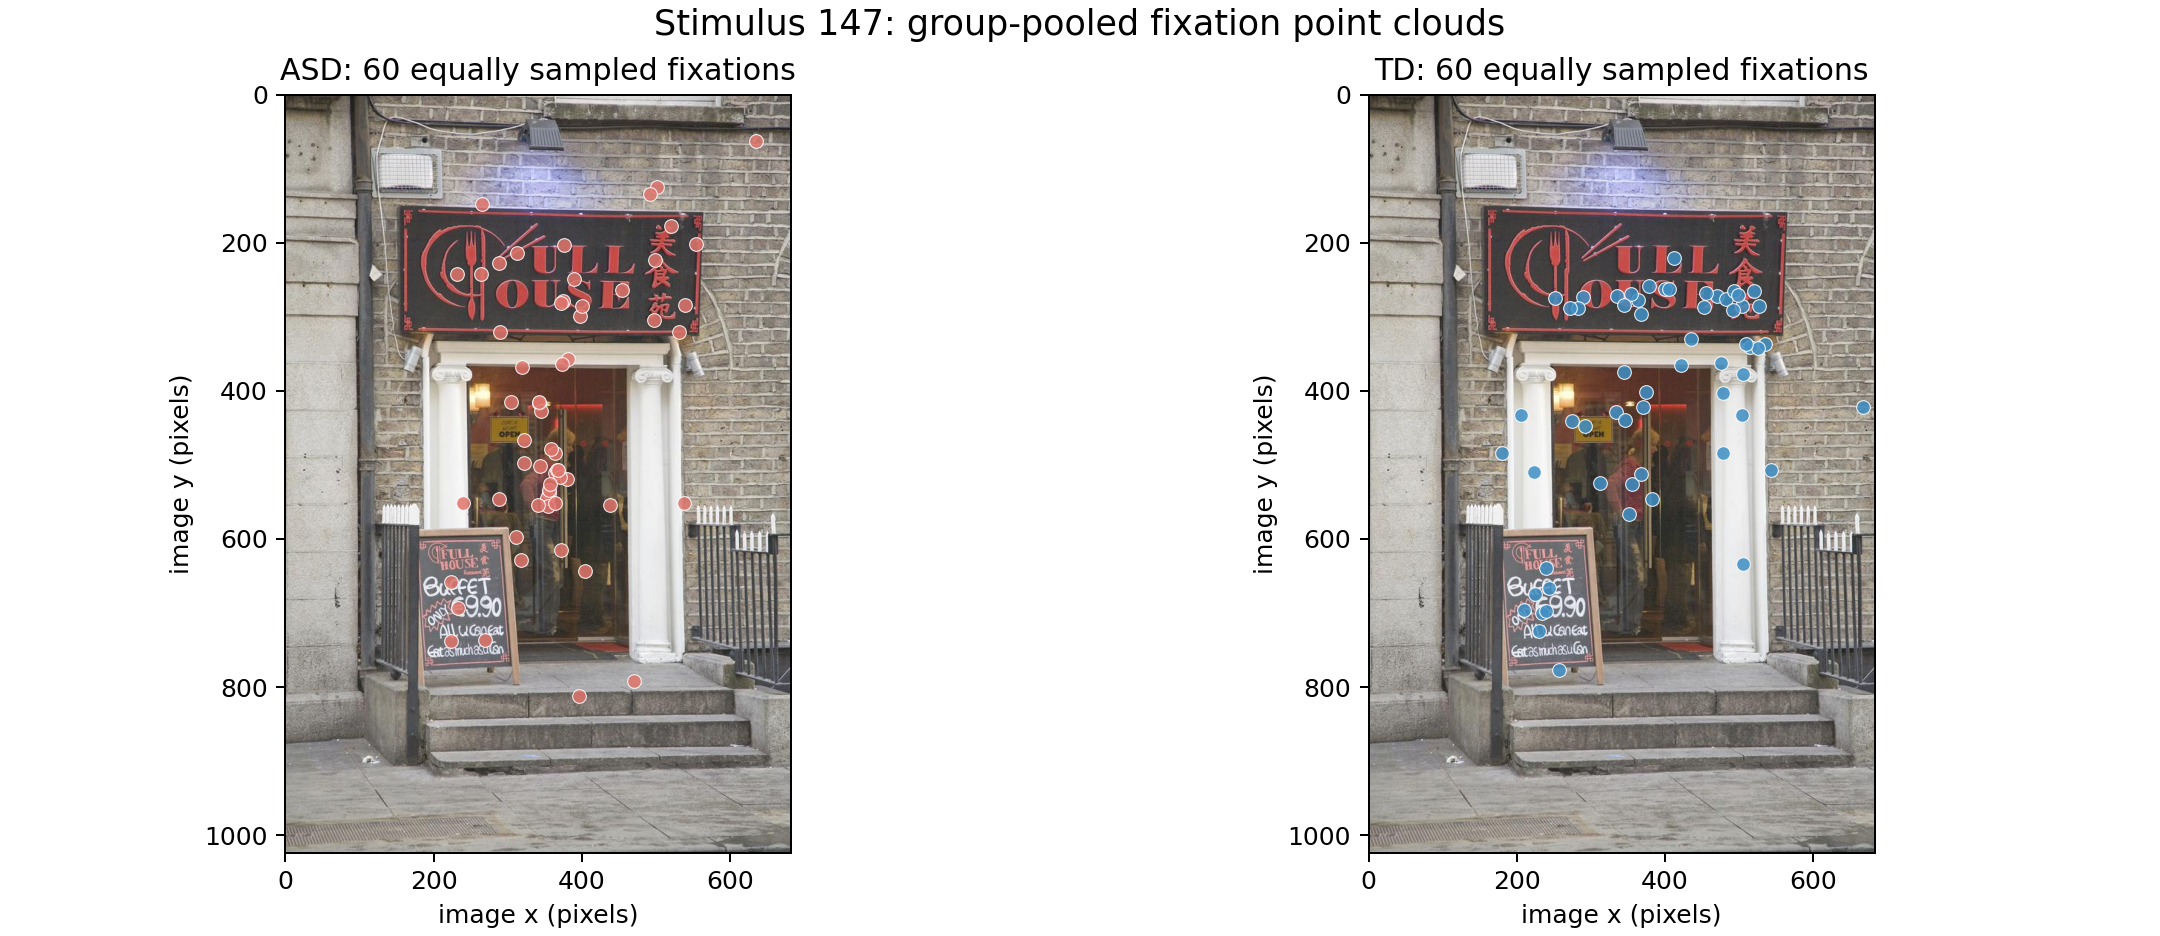
\includegraphics[width=\textwidth]{figures/gaze_point_cloud_example.png}
  \caption{A representative matched pair of group-pooled fixation point
  clouds.  The same stimulus is shown for \ASD{} and \TD{}, with 60 points in
  each panel.}
  \label{fig:cloud}
\end{figure}

Figure~\ref{fig:barcode} displays the associated $H_0$ and $H_1$ barcodes.
Longer bars represent structures that persist over a larger range of spatial
scales.  The single example should not be interpreted as a group estimate;
group conclusions use all 287 matched images and all 20 repetitions.

\begin{figure}[htbp]
  \centering
  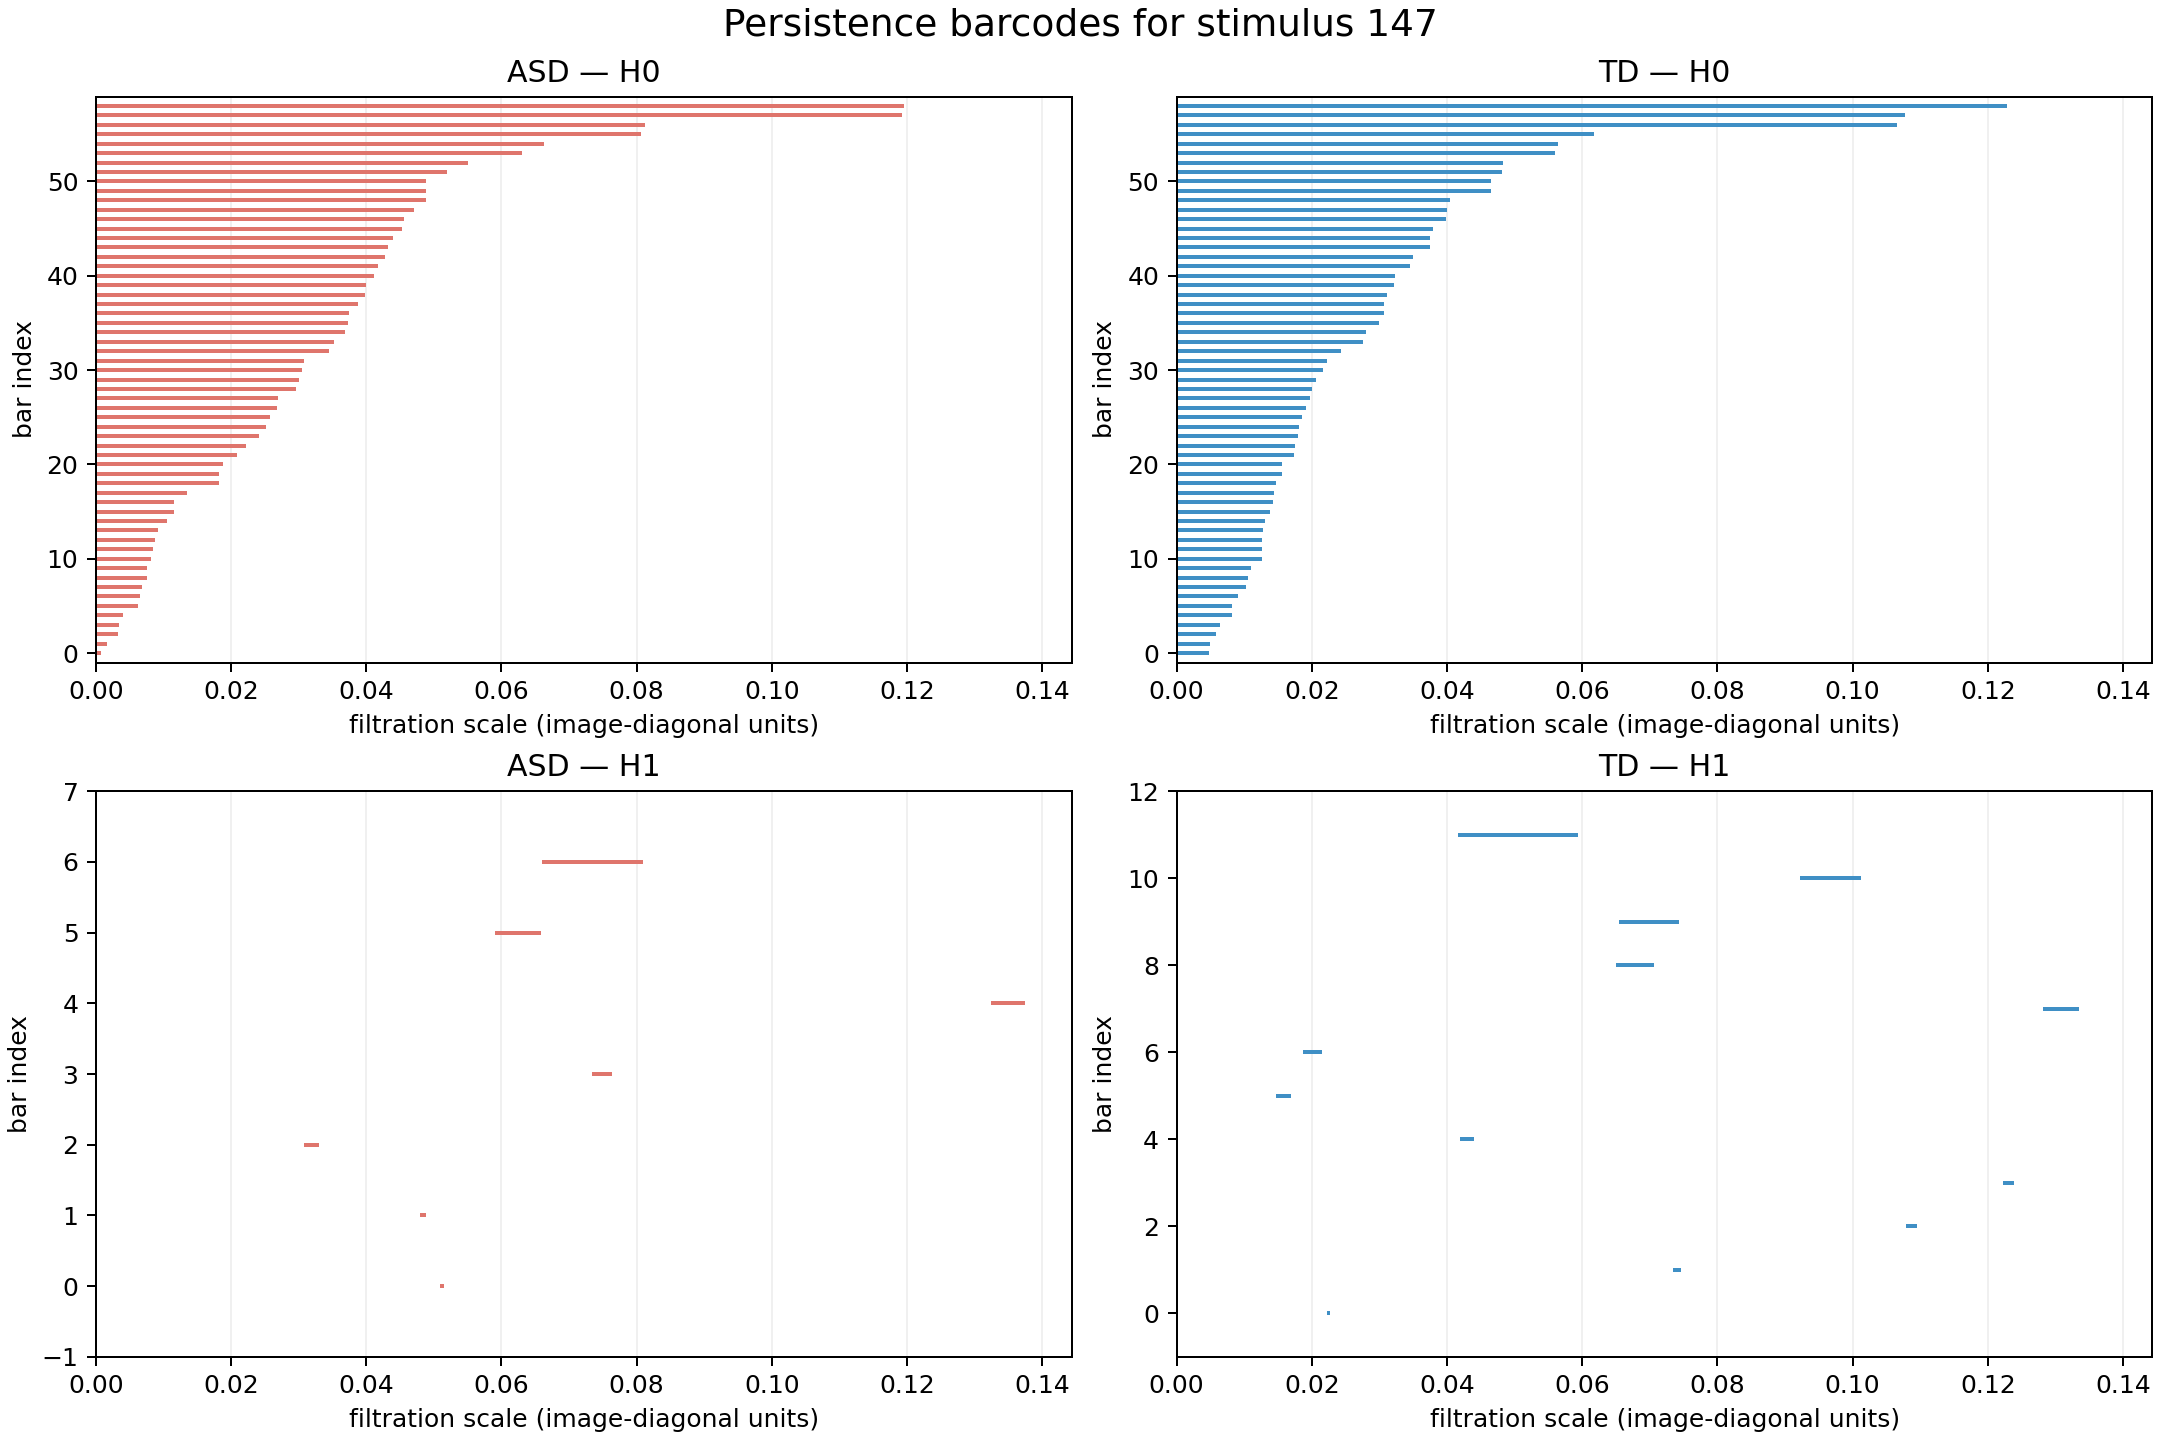
\includegraphics[width=0.95\textwidth]{figures/persistence_barcode_example.png}
  \caption{Persistence barcodes for the representative sample.  The top row
  shows finite $H_0$ intervals and the bottom row shows $H_1$ intervals.}
  \label{fig:barcode}
\end{figure}

\subsection{Group-mean stable-rank curves}

The mean stable-rank curves are shown in Figure~\ref{fig:stable}.  In $H_0$,
the \ASD{} curve is generally above the \TD{} curve across intermediate
lifetime thresholds and decays more slowly.  This indicates that more finite
components remain separated over larger spatial scales.  The $H_1$ curves are
lower and concentrated near short lifetimes; the \ASD{} mean is again
slightly higher, but image-level variability is substantial.

\begin{figure}[htbp]
  \centering
  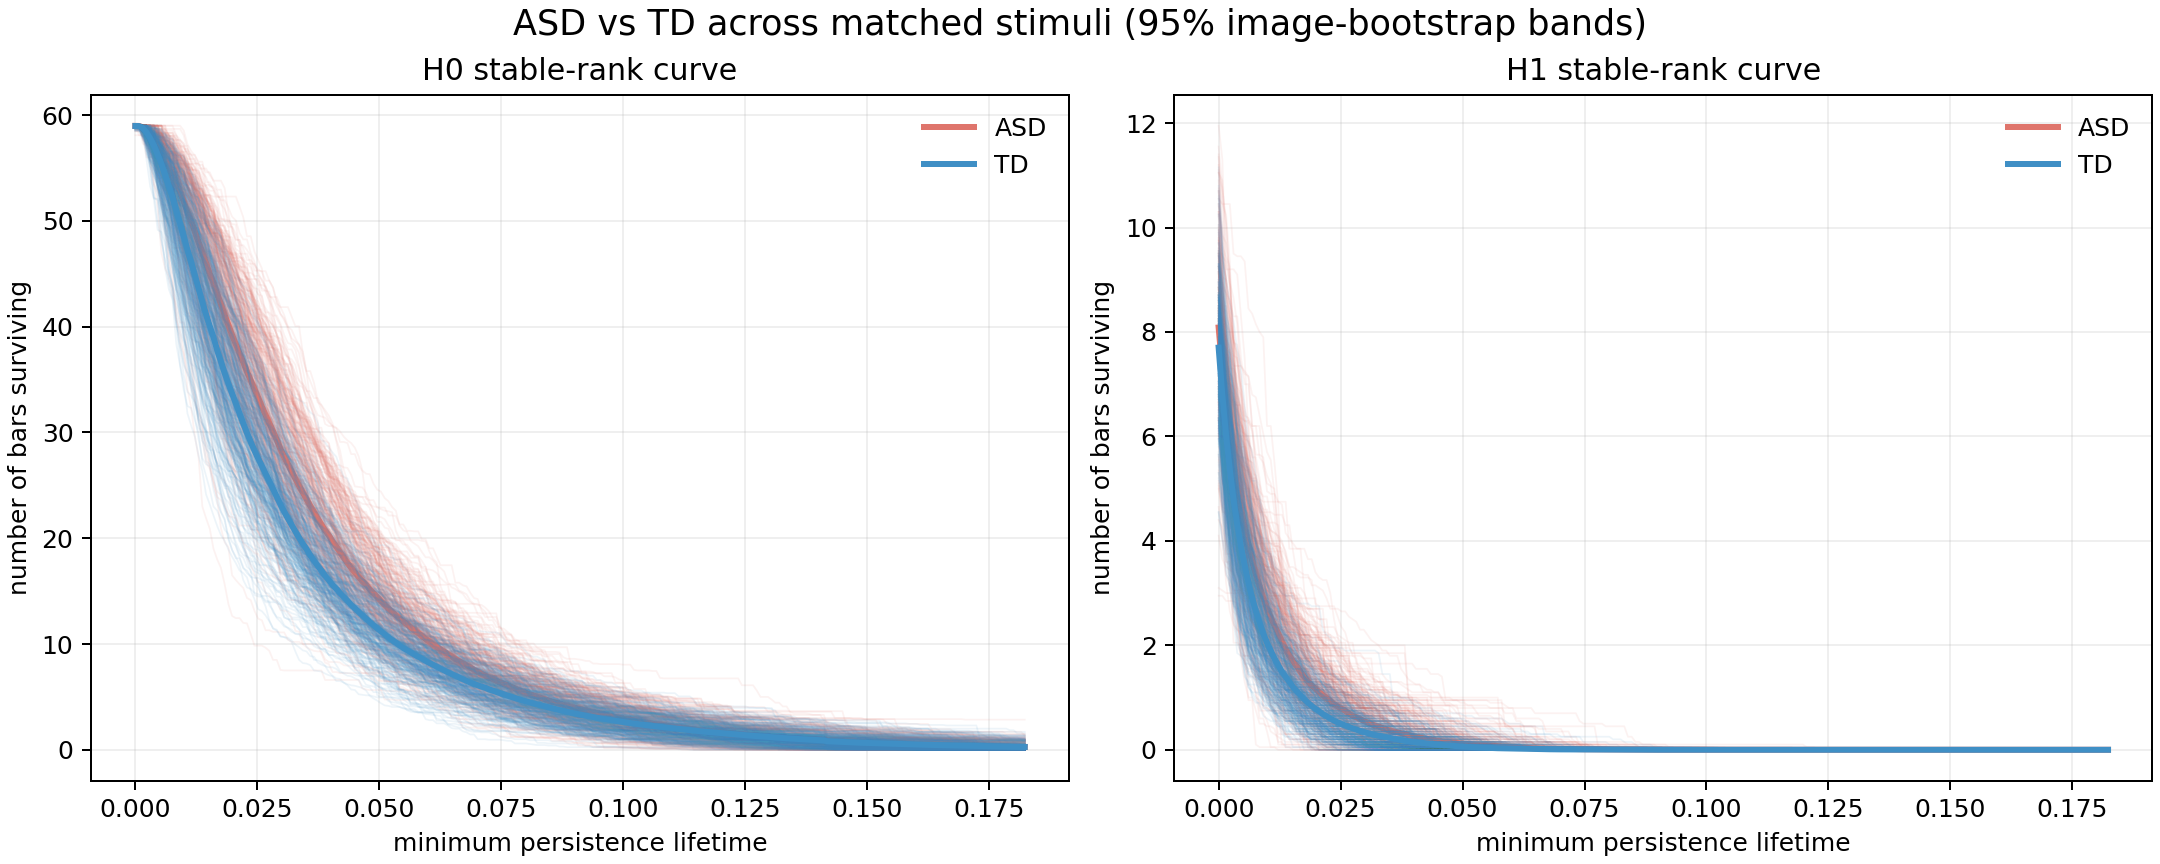
\includegraphics[width=\textwidth]{figures/stable_rank_group_comparison.png}
  \caption{Image-level stable-rank curves (thin lines), group means (thick
  lines), and 95\% image-bootstrap bands.  Repetitions were averaged within
  image before any between-image aggregation.}
  \label{fig:stable}
\end{figure}

\subsection{Paired scalar summaries}

Table~\ref{tab:results} summarizes the matched image-level comparisons.  \ASD{}
has greater mean dispersion ($d_z=0.865$) and greater $H_0$ total persistence
($d_z=0.948$).  In contrast, the maximum $H_0$ lifetime is nearly identical
between groups: its bootstrap interval crosses zero and its Holm-adjusted
$p$-value is 0.409.  The primary $H_0$ difference is therefore cumulative
across many bars rather than caused by one exceptionally persistent component.

The $H_1$ feature count, total persistence, and maximum persistence are also
higher for \ASD{}.  Their effects are smaller than the $H_0$ total-persistence
effect and should remain exploratory because $H_1$ is more sensitive to local
sampling geometry.

\begin{table}[htbp]
\centering
\small
\caption{Paired stimulus-level results.  Differences are \ASD{} minus \TD{}.
Confidence intervals resample matched images; $p_{\mathrm{Holm}}$ adjusts six
exploratory paired tests.}
\label{tab:results}
\begin{tabular}{lrrrrr}
\toprule
Feature & \ASD{} & \TD{} & Difference [95\% CI] & $d_z$ & $p_{\mathrm{Holm}}$\\
\midrule
Dispersion & 0.1513 & 0.1331 & 0.0181 [0.0157, 0.0206] & 0.865 & $<10^{-15}$\\
$H_0$ total persistence & 2.2164 & 1.9490 & 0.2674 [0.2356, 0.3019] & 0.948 & $<10^{-15}$\\
$H_0$ maximum persistence & 0.1573 & 0.1553 & 0.0021 [$-0.0028$, 0.0069] & 0.049 & 0.409\\
$H_1$ feature count & 8.0859 & 7.7009 & 0.3850 [0.2047, 0.5657] & 0.247 & $7.37\times10^{-5}$\\
$H_1$ total persistence & 0.0803 & 0.0626 & 0.0177 [0.0147, 0.0209] & 0.655 & $<10^{-15}$\\
$H_1$ maximum persistence & 0.0303 & 0.0250 & 0.0053 [0.0040, 0.0066] & 0.477 & $5.50\times10^{-14}$\\
\bottomrule
\end{tabular}
\end{table}

\begin{figure}[htbp]
  \centering
  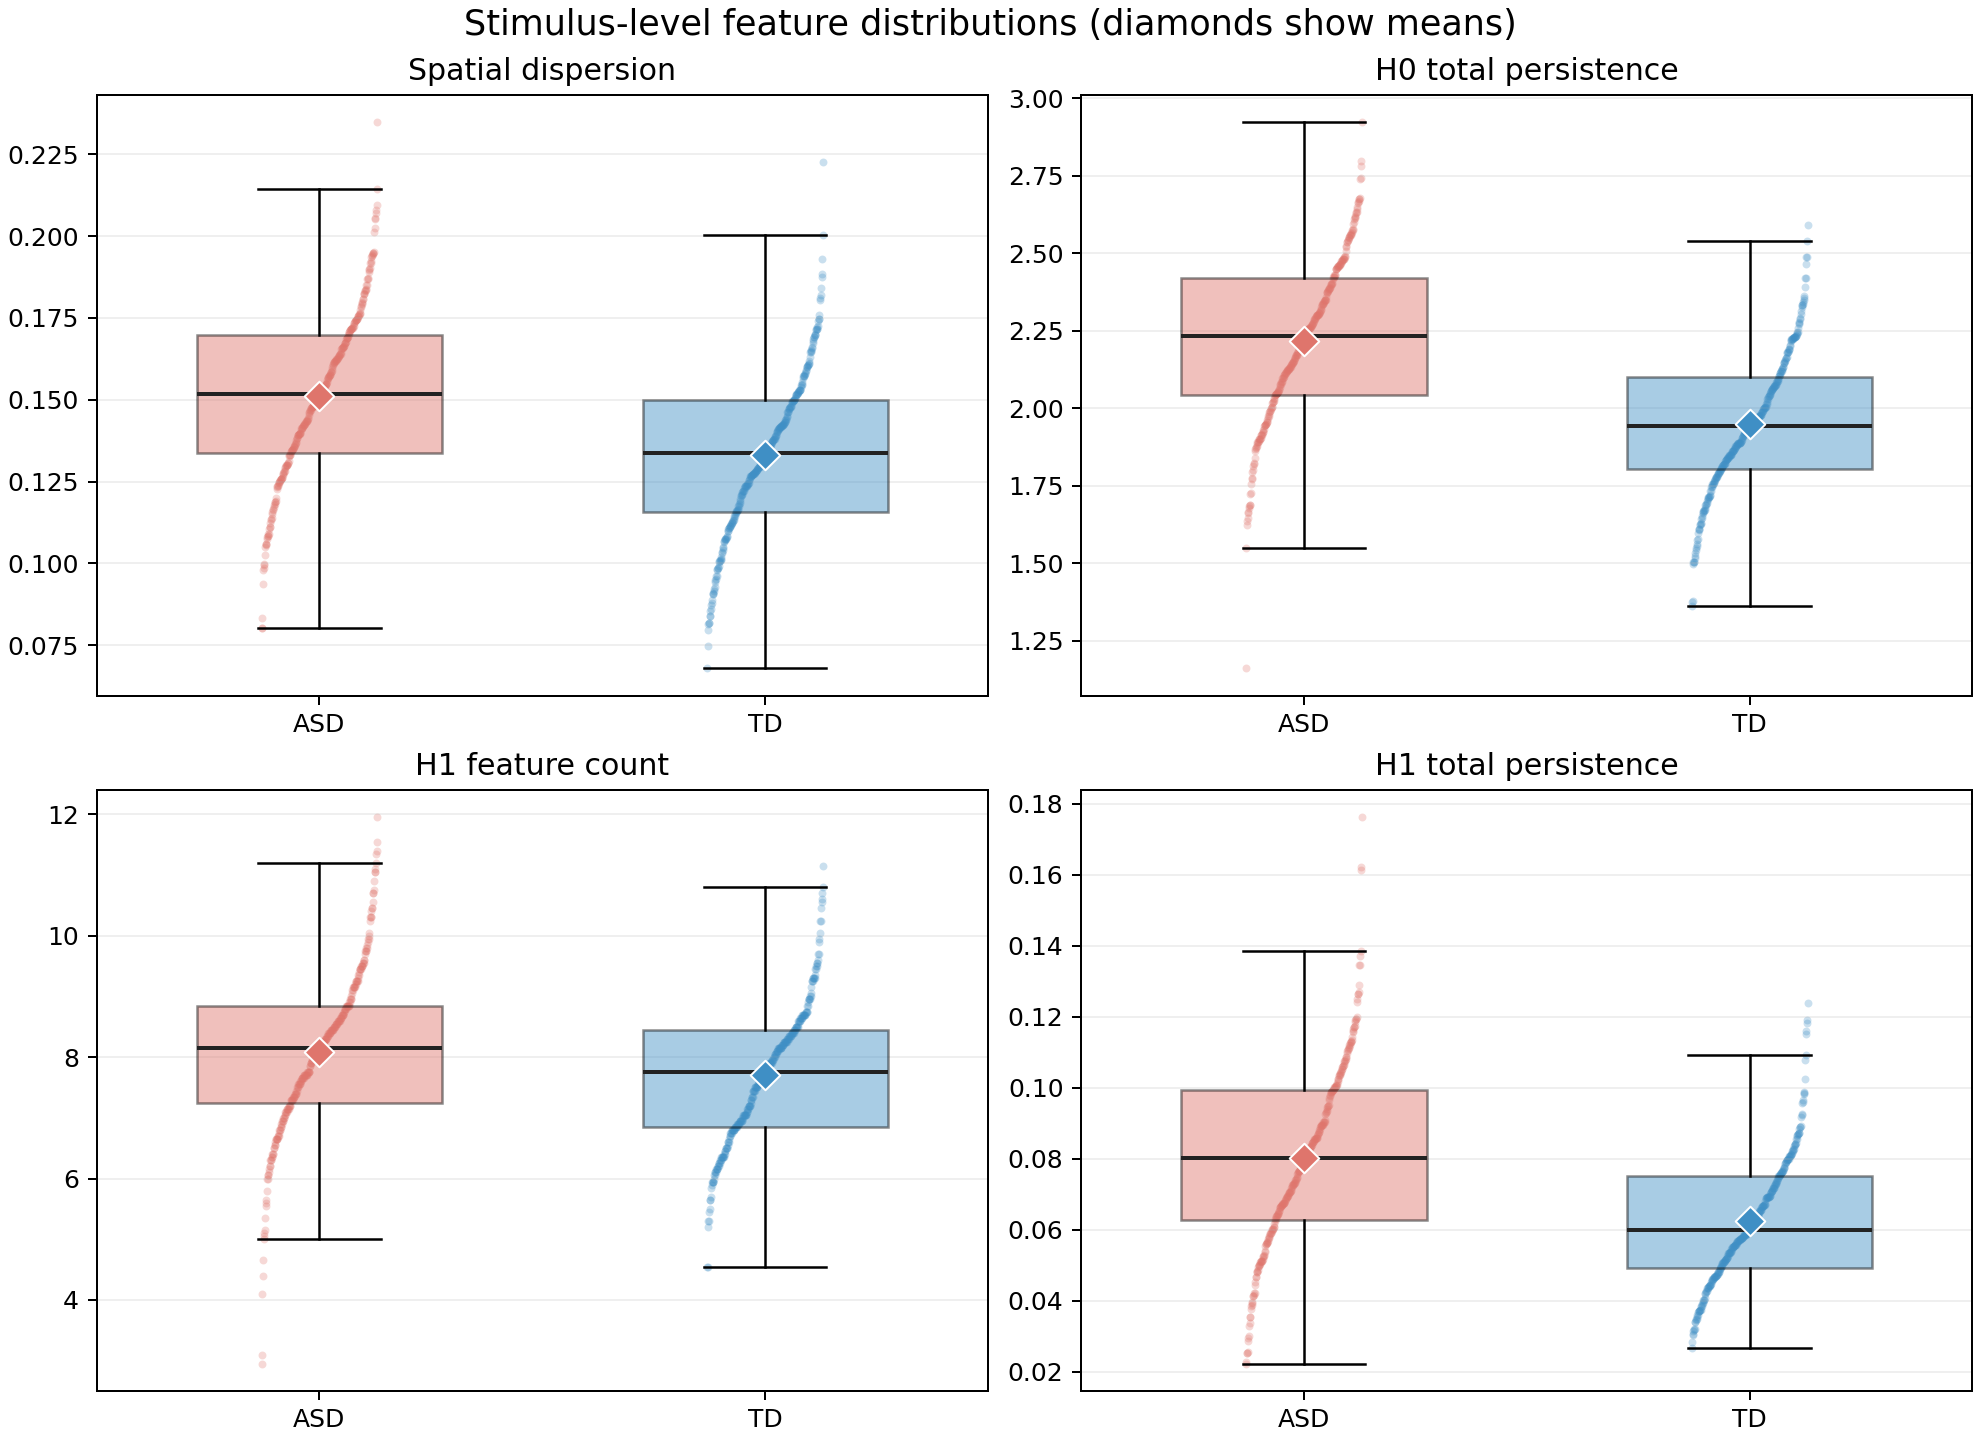
\includegraphics[width=0.94\textwidth]{figures/feature_comparisons.png}
  \caption{Stimulus-level distributions of selected non-topological and
  topological summaries.  Diamonds indicate group means.}
  \label{fig:features}
\end{figure}

\subsection{How much does $H_0$ add beyond dispersion?}

Within groups, $H_0$ total persistence correlates with centroid dispersion
($r=0.717$ for \ASD{} and $r=0.637$ for \TD{}).  More importantly, the paired
\ASD--\TD{} difference in $H_0$ total persistence correlates with the paired
dispersion difference ($r=0.656$).  The primary TDA result therefore largely
reflects a multiscale form of overall spatial dispersion.  This is not a flaw:
for a fixed number of points, finite $H_0$ persistence is closely related to
the edge lengths of a minimum spanning tree.  It does, however, mean that the
$H_0$ result should not be presented as independent evidence for a novel
topological biomarker.

The corresponding difference correlation is smaller for $H_1$ total
persistence ($r=0.391$), suggesting that $H_1$ contains some geometric
information not reducible to radial dispersion alone.  Its interpretation is
nevertheless less stable and less directly linked to a behavioural mechanism.

\section{Discussion}

The final 60-point, 20-repetition analysis supports a clear stimulus-level
pattern: group-pooled \ASD{} fixations are more spatially dispersed than
group-pooled \TD{} fixations on the same images.  Persistent homology captures
this pattern without selecting one arbitrary clustering radius.  The higher
and slower-decaying \ASD{} $H_0$ stable-rank curve shows that the difference is
present across a range of persistence lifetimes.  The absence of a stable
difference in maximum $H_0$ persistence further indicates a distributed shift
across the point cloud rather than a single extreme outlier or isolated gaze
region.

TDA is useful here because it supplies a multiscale, coordinate-free summary
of point-cloud organization and allows $H_0$ and $H_1$ to be studied in a
common framework.  It does not automatically outperform simpler statistics.
Indeed, the correlation analysis shows that the strongest $H_0$ finding is
closely connected to conventional dispersion.  The defensible conclusion is
therefore not that topology uniquely classifies autism, but that persistent
homology provides a robust multiscale description of a group-level spatial
dispersion difference.

\subsection{Limitations}

\begin{enumerate}
  \item The public release does not provide a persistent participant ID across
  images.  Fixations are pooled by image and group, preventing individual-level
  inference or classification.
  \item The same cohort viewed many stimuli.  Treating images as the bootstrap
  and testing unit measures consistency across the stimulus set but does not
  replace inference over independently sampled children.  Very small
  image-level $p$-values must not be interpreted as clinical significance.
  \item The 60-point threshold excludes 13 stimuli and discards valid points
  from larger pools.  Repeating the sampling reduces dependence on one subset
  but does not eliminate selection effects.
  \item Duration and temporal order are excluded.  Consequently, $H_1$ holes
  are spatial gaps, not evidence of circular gaze motion or switching.
  \item Stimulus semantics are not modelled.  Coordinates alone cannot reveal
  whether a fixation lies on a face, eye, object, or background region.
  \item Age, recording quality, and other child-level covariates cannot be
  controlled with the released organization used here.
\end{enumerate}

Future work should use persistent participant identifiers and a hierarchical
model with children and stimuli as crossed factors.  Sensitivity analyses over
point caps, semantic areas of interest, duration-weighted constructions, and
order-aware scanpath topology would help separate spatial dispersion from
attention dynamics.

\section{Conclusion}

Using balanced point clouds and matched stimuli, the analysis finds that \ASD{}
group fixation locations are, on average, more spatially dispersed and have
greater cumulative $H_0$ persistence than \TD{} locations.  $H_1$ differences
are present but secondary.  The results demonstrate a meaningful use of TDA:
the stable-rank curves summarize group differences across spatial scales.
They do not establish a participant-level diagnostic signature, and the
dominant $H_0$ effect should be understood primarily as a multiscale expression
of dispersion.

\section*{Reproducibility}

The final analysis uses random seed 2956 and can be reproduced from the project
directory with:
\begin{verbatim}
python3 run_2d_pipeline.py --point-cap 60 --min-points 60 \
  --repeats 20 --bootstrap 2000 --seed 2956 \
  --output-dir output/final_60x20
python3 summarize_final_analysis.py
\end{verbatim}
The Saliency4ASD dataset record is available at
\url{https://zenodo.org/records/13960770}.  Raw data are not redistributed by
this report.

\begin{thebibliography}{9}

\bibitem{duan2019}
H. Duan et al.
\newblock Saliency4ASD: Challenge, Dataset and Tools for Visual Attention
Modeling for Autism Spectrum Disorder.
\newblock \emph{Proceedings of ACM Multimedia Systems Conference}, 2019.

\bibitem{edelsbrunner2010}
H. Edelsbrunner and J. Harer.
\newblock \emph{Computational Topology: An Introduction}.
\newblock American Mathematical Society, 2010.

\bibitem{ghrist2008}
R. Ghrist.
\newblock Barcodes: The persistent topology of data.
\newblock \emph{Bulletin of the American Mathematical Society}, 45(1):61--75,
2008.

\bibitem{course}
W. Chach\'olski.
\newblock \emph{SF2956 Topological Data Analysis: Course Notes}.
\newblock KTH Royal Institute of Technology, 2026.

\end{thebibliography}

\end{document}
